\section{Spikes}
\ghnote{Antar dette blir et Torbjoern-kapittel.}

\ghnote{Tekst under klippet fra bokkapittel. Tenker at vi trenger en intro her som forklarer dette.}
Extracellular potentials measured within neural tissue are often split into two separate frequency domains, which reflect different aspects of the underlying neural activity. The low frequency part, the local field potential (LFP), is thought to mostly reflect synaptic input to populations of pyramidal cells, while the high-frequency part, the multi-unit activity (MUA), reflects the population spiking activity (Fig.~\ref{fig:LFP_MUA}).
\begin{figure}[!ht]
\begin{center}
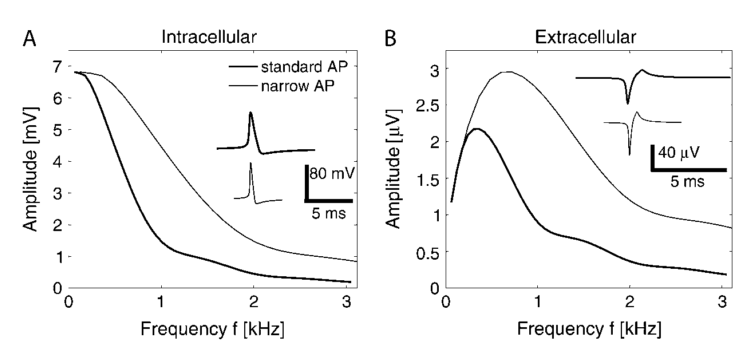
\includegraphics[width=0.6\textwidth]{Figures/eap_illustration.png}
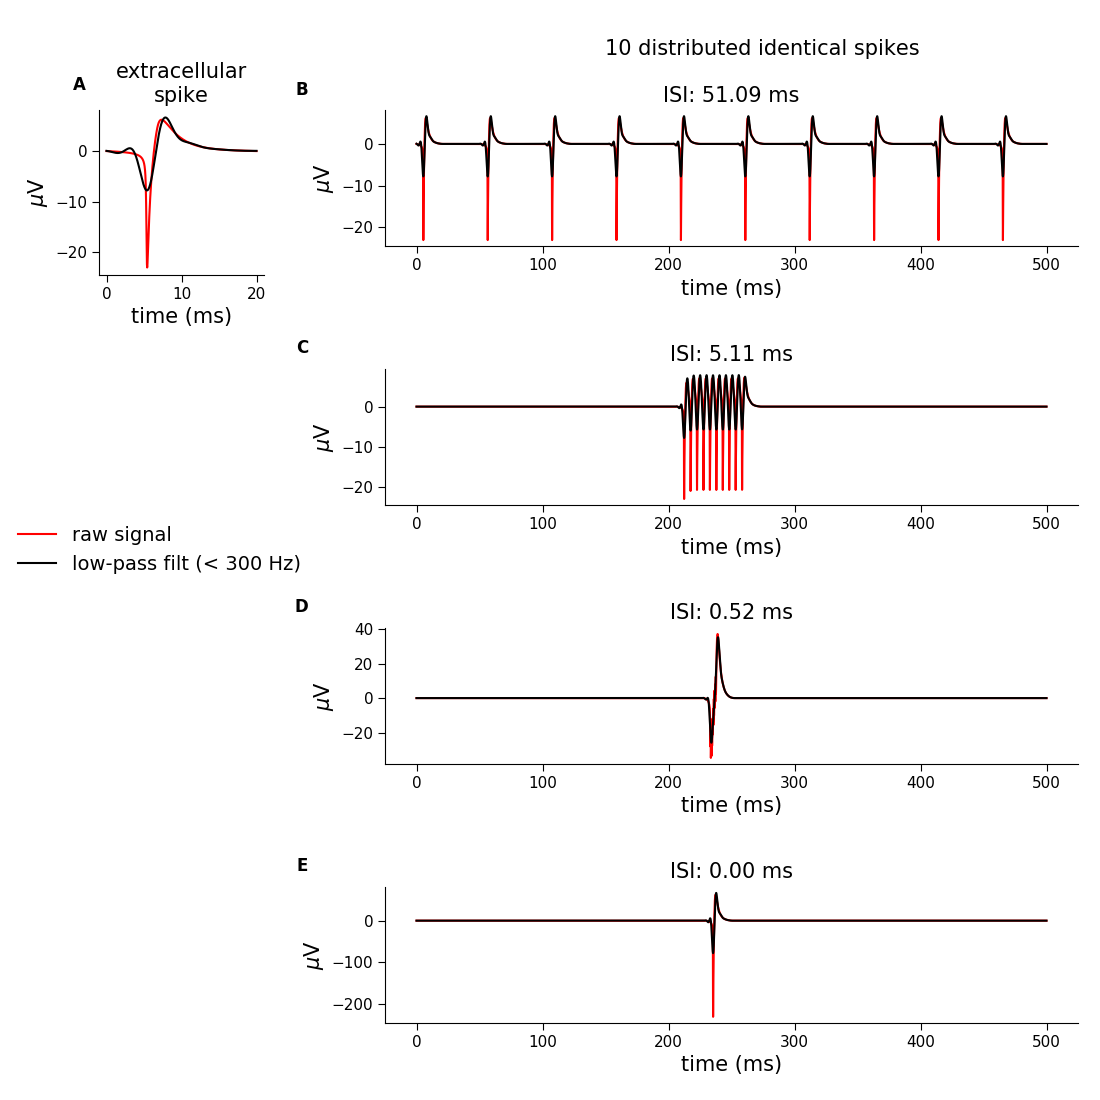
\includegraphics[width=0.6\textwidth]{Figures/LFP_spike_effect_test_300Hz.png}
\end{center}
\caption{\textbf{Potential EAP figures} 
} Common missconception that spikes only have frequency content above a few hundred Hz. Delta pulse have flat frequency spectrum.
\label{fig:freq_dep}
\end{figure}

\subsection{Spikes in neurons with passive dendrites} 
Kjernereferanse: \citep{Pettersen2008a}

Perhaps start this by showing membrane potentials for cells with passive dendrites. 
Then show extracellular signatures.

\subsection{Spikes in neurons with active dendrites} 
Kjernereferanse: \citep{Gold2006}
Perhaps start this by showing membrane potentials for cells with active dendrites. 
Then show extracellular signatures.

\subsection{Multi-unit activity (MUA)} 
Kjernereferanse: \citep{Pettersen2008}

\subsection{Insights from MUA studies} 
\ghnote{I added this kind of subsection to most of the Part 2 - sections. I thought it might be an idea to finish the MUA, LFP, ECoG and EEG sections with summaries of what these modalities typically tell us, i.e. in terms of (i) what aspects of neural activity they reflect (spikes, synaptic inputs, dendritic ion channels, which ion channels, which kind of neurons, something on network structure, cell orientation, cortical folding etc.), and what what they can tell us about cognitive states (attentive, drowsy etc.). I am not sure about this idea, though. Maybe it will be too challenging to get an overview over the literature - we dont want to put the entire Nunez-book into the EEG-chapter.}
